\section{Clock Frequency Measurement}
After installing the resistor and capacitor in the appropriate terminals, the
system was powered with zero input so that students could observe the waveform
that appeared at pin four of the ADC, i.e. the internal clock frequency.  An
oscilloscope screenshot of this signal is shown in Figure~\ref{f:clock}.
%
\begin{figure}[H]
\centering
	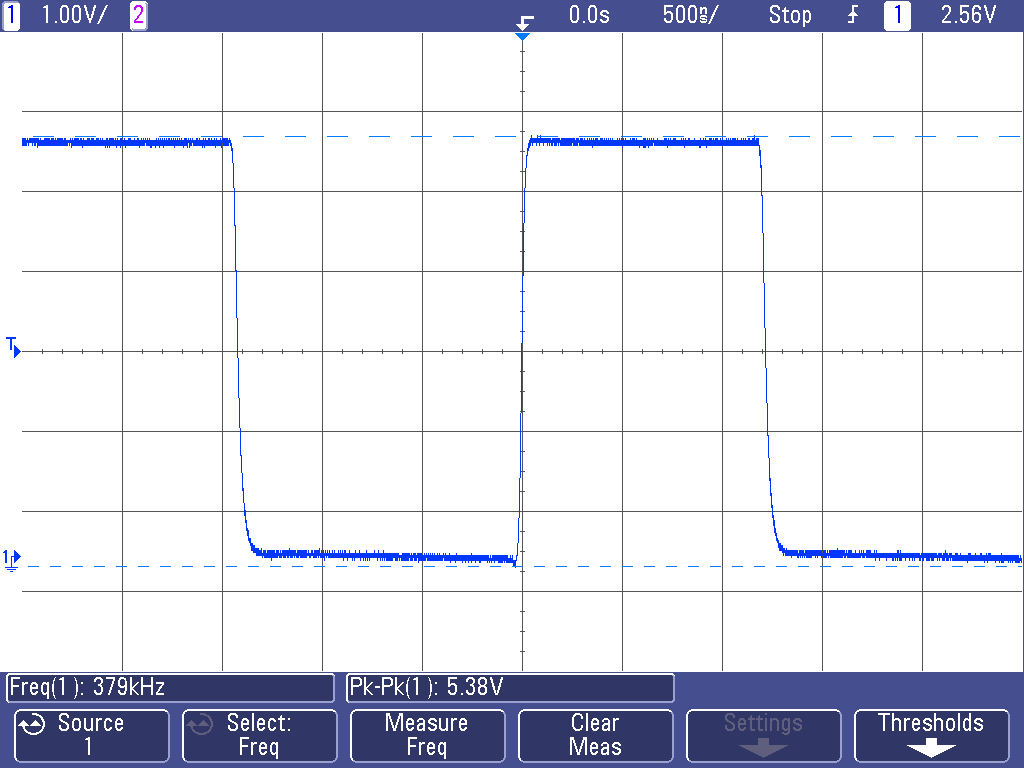
\includegraphics[width=.8\textwidth]{img/shot/RC_clock_shot.png}
	\parbox{.8\textwidth}{
	\caption[Internal clock waveform]{Captured signal of the system's internal
	clock.  Note the drastic decrease in frequency compared to the target
	frequency.}
	\label{f:clock}}
\end{figure}
%
As is shown, the clock frequency of the ADC is only about half of the intended
frequency.  This is most easily attributed to additional intrinsic capacitances
within the circuit board.  Despite the severely decreased clock frequency, all
other students observed a similar phenomenon in their systems, and the
instructor confirmed that this is a known flaw in the design.  As such, the
evaluation of the ADC was allowed to proceed with an internal clock frequency
of~\SI{379}{\kilo\hertz}.
